\section{Geant4シミュレーションによる実機シミュレーション}
実機では2$-$16\space$\si{GeV/c}$の$\pi$/K/pの識別が必要となるため、
実際に$\pi$、K、pを入射させ、識別効率の確認を行った。
ただし、今回は輻射体としてガスを用いたテスト実験は行なっていないため、エアロゲルのみを用いたシミュレーションを行った。
エアロゲルでは、2$-$6\space$\si{GeV/c}$の$\pi$/k、2$-$10\space$\si{GeV/c}$のK/pを識別する必要があるため、
この範囲での識別性能を確認した。

\subsection{ジオメトリ}
図\ref{fig:ActualSimulationSetup}に実機シミュレーションのジオメトリの概略図を示す。
球面鏡、検出面の角度は設計値の$10^{\circ}$、$20^{\circ}$に設定した。
球面鏡は曲率半径$\SI{3000}{mm}$とし、外径は$\SI{1100}{mm}\times\SI{1100}{mm}$とした。
検出面は基本的には先ほどのシミュレーションと同様の$\SI{50}{mm}$コーンとMPPCで構成したが、
テスト実験とは違い、図\ref{fig:ActualSimulationDetectorPlane}に示すように$22個(縦)\times23個(横)$のコーンをハニカム構造で設置した。
エアロゲルの中心から球面鏡の表面、球面鏡の表面から検出面のコーン入口までの距離はどちらも
球面鏡の焦点距離である$\SI{1500}{mm}$とした。
ビームは2$-$10\space$\si{GeV/c}$の$\pi$、K、pを$\SI{200}{MeV/c}$のステップで入射させた。
その際に、チャームバリオン分光実験に用いる飛跡検出器の分解能$\SI{1}{mrad}$をビームの角度分布の$\sigma$として設定した。
コーン型ライトガイドの反射率は、先ほど決定した0.675とし、MPPCの検出効率とは$\rm{V_{ov}}\SI{4}{V}$の値を使用し、
Dark currentのレートは$\rm{V_{ov}}\SI{4}{V}$の場合の全CHの平均値とした。
今回のシミュレーションではエアロゲルは1つとし、サイズは$\SI{146}\times\SI{146}{mm}\times\SI{50}{mm}$、屈折率1.04、
透過長は波長$\SI{400}{nm}$に対して$\SI{55.0}{mm}$で波長依存性を考慮して設定し、吸収長は波長に依らず$\SI{5500}{mm}$とした。

\begin{figure}
  \centering
  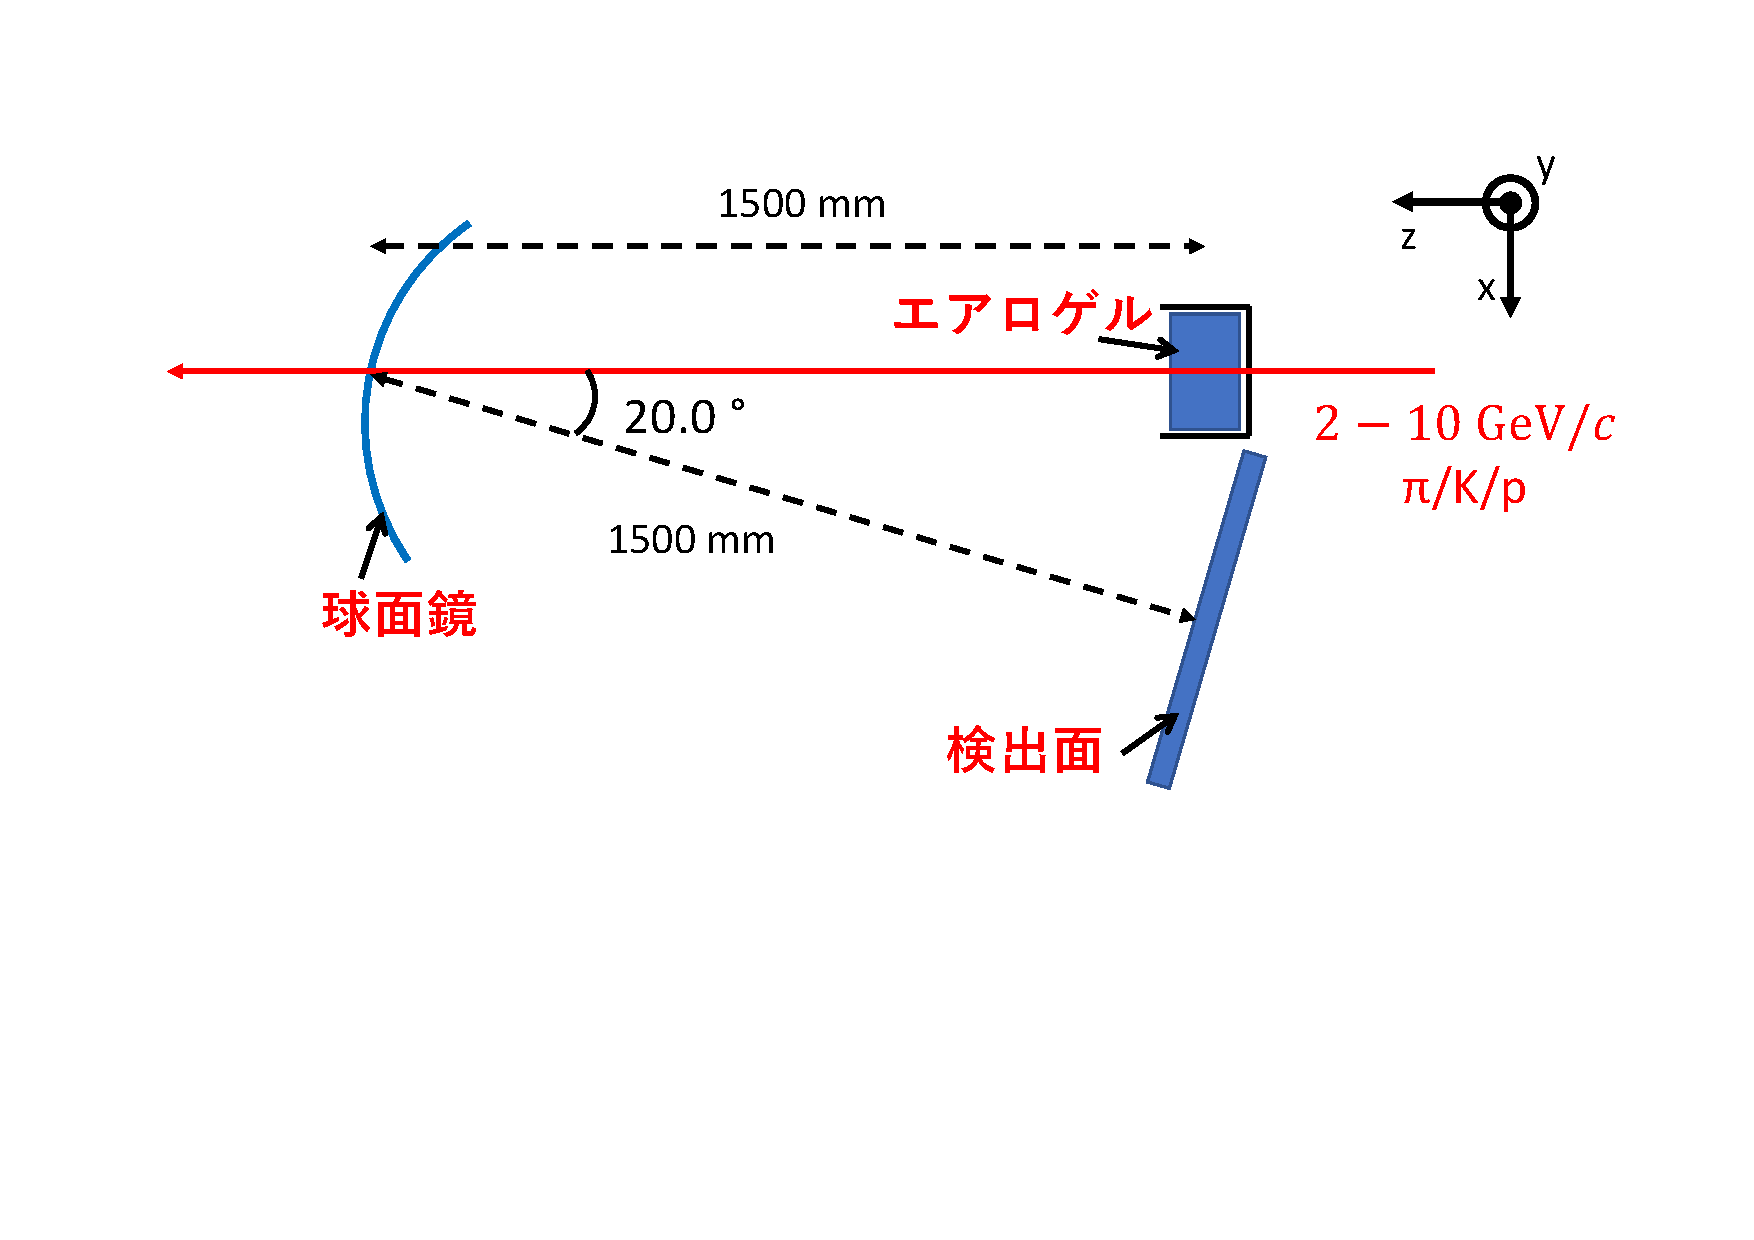
\includegraphics[width=15cm]{images/chapter4/ActualSimulationSetup.pdf}
  \caption{
    実機シミュレーションジオメトリの概略図。
  }
  \label{fig:ActualSimulationSetup}
\end{figure}


\begin{figure}
  \centering
  \includegraphics[width=10cm]{images/chapter4/ActualSimulationDetectorPlane.pdf}
  \caption{
    実機シミュレーションの検出面を正面から見た様子。サイズは$\SI{1100}{mm}(縦)\times\SI{1003}{mm}(横)$。
  }
  \label{fig:ActualSimulationDetectorPlane}
\end{figure}

